
%(BEGIN_QUESTION)
% Copyright 2012, Tony R. Kuphaldt, released under the Creative Commons Attribution License (v 1.0)
% This means you may do almost anything with this work of mine, so long as you give me proper credit

Analyse this relay ladder-logic (RLL) program written for a Koyo CLICK PLC, designed to send an ASCII-encoded text message to a data terminal (e.g. a personal computer running a terminal emulator program, ready to display any text sent to it by the PLC over a serial data cable) whenever an alarm switch detects a high-temperature condition in a furnace:

$$\includegraphics[width=15.5cm]{i03743x01.eps}$$

Answer the following questions about this PLC program:

\begin{itemize}
\item{} Based on what you see here, is the high-temperature alarm switch sending the signal to the PLC electrically {\it NO} or is it {\it NC}?  Is it even possible to tell, or do we need more information?
\vskip 10pt
\item{} Why is an edge-transition contact instruction used on the {\tt X8} input bit, rather than a normal contact instruction?
\vskip 10pt
\item{} Modify the program so that it will work well without having to use an edge transition contact instruction.
\vskip 10pt
\item{} Modify the program so that it will only send no more than one message per 10 minutes, even if the high-temperature switch keeps tripping and resetting at a frequency faster than that.
\end{itemize}

\underbar{file i03743}
%(END_QUESTION)





%(BEGIN_ANSWER)

We can tell that the high-temperature switch must have normally-open (NO) contacts, because it is on the {\it positive} edge transition that the PLC transmits the message (i.e. when the temperature switch {\it closes}).  Thus, the switch must transition from open to close as temperature rises, making it an NO contact.

\vskip 10pt

The edge-transition contact instruction is used so that the PLC does not continually repeat the message if a high-temperature condition continues unabated over time.

\vskip 10pt

Modification of program to avoid using edge-transition instruction:

$$\includegraphics[width=15.5cm]{i03743x02.eps}$$

{\it Note: the order in which these ladder-logic rungs appear in this example are essential to the program operating properly.  The ``Send'' rung \underbar{must} precede the interlock ({\tt C3} coil) rung.}

\vskip 10pt

The program shown here does the same thing as a positive edge-detect instruction, and it does so by exploiting the scan order of the PLC.  When {\tt X8} first transitions from low to high (0 to 1) and the PLC scans the program from top to bottom, the first rung is executed because {\tt X8} = 1 and {\tt C3} = 0.  After the second rung scans, however, bit {\tt C3} becomes set, preventing any further executions of the Send instruction in the top rung.

\vskip 10pt

\filbreak

Modification of program to avoid nuisance alarm messages:

$$\includegraphics[width=15.5cm]{i03743x03.eps}$$

%(END_ANSWER)





%(BEGIN_NOTES)


%INDEX% PLC, ladder logic program analysis and explanation (Koyo CLICK)

%(END_NOTES)


